% RQ3
\section{Ranking}
\label{sec:toolranking}
% Most important:
% Finding the top performing tool is most important, then low MSE for that top performing
% Confidence in automation
% 

Now that a predictor for future error detection tool performance is introduced, the goal of an estimated ranking of tools with respect to their performance will be discussed.
~\\As an absolute score is helpful to know with a single tool at your disposal, a ranking or recommendation of tools and their strategies would be of greater use for the end-user. The question proposed here is to see if such a ranking could be made, ranking the better performing tools higher in the ranking. This also allows for other metrics to experiment with. The regressors (estimators) used in section \ref{sec:performanceprediction} could now also be optimized using information retrieval ranking scores. This might result in different distinguishing features found by the regression models and shows the possible flexibility of these models (if it is possible to get good rankings).
The flow of the ranking is shown in figure \ref{fig:method_ranking}.

\begin{figure}
    \centering
    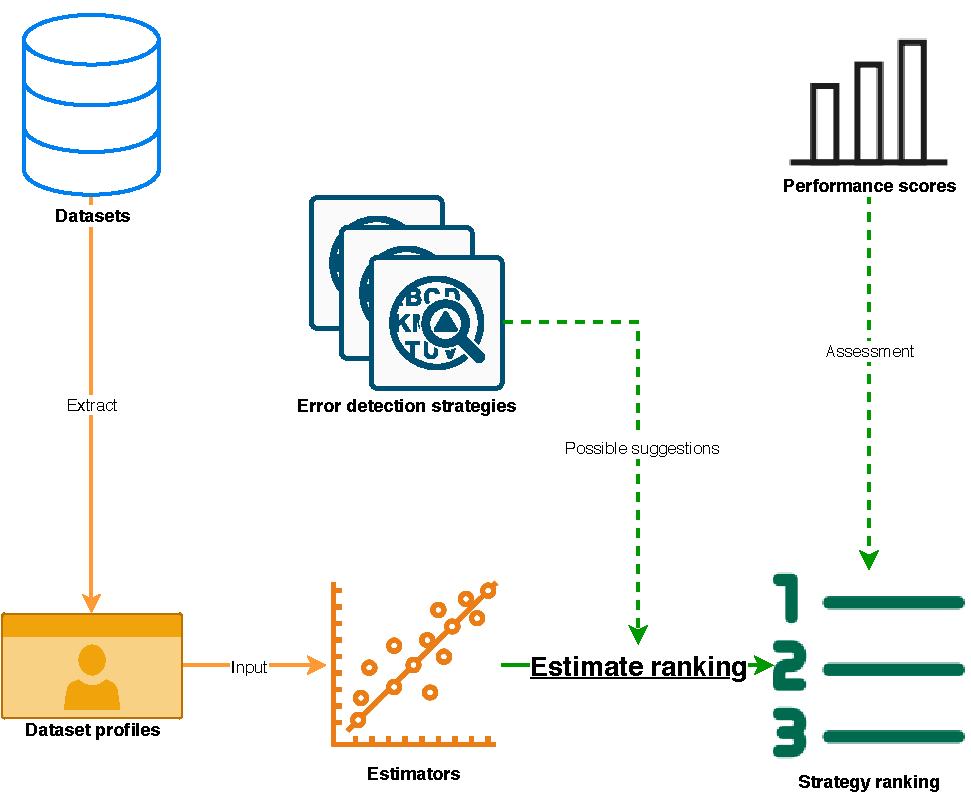
\includegraphics[width=0.9\textwidth]{thesis/Figures/Method/PerformanceEstimation-Ranking.pdf}
    \caption{Flow of the estimation of strategy ranking}
    \label{fig:method_ranking}
\end{figure}

\subsection{Method of ranking}
A user should be able to retrieve an estimated ranking of high performing strategies without running these tool on an unseen dataset. A ranking should be $K$ strategies long, with a predefined $K$. It should be so that a user can a variety of tools and configurations to pick from. To evaluate whether it is possible to create such an estimated ranking, two types of rankings will be made and scored. First, a ranking based on finding the best tool for the dataset will be created. Then, a ranking based on finding the best configuration for a tool will be created.
To test if estimated strategy ranking is viable, this section will focus on F1 estimation and ranking only. 
\\To generate an estimated ranking for a new unseen dataset, the data profile as described in section \ref{subsec:dataprofiles} is created. Then, all estimators as found by section \ref{subsec:estimatorselection} are given this data profile as input, generating estimated scores for all strategies $s \in S$. These estimated scores (like a single column in table \ref{tab:estimatedscores}) are then sorted. Depending on the task (best tool or best configuration), the results are filtered and only the top suggestions are kept.

\paragraph{Best tool} The best tool configuration is similar to the one shown in table \ref{tab:ranking_best_tool}. For the 6 tools that are used in this research, 1 configuration will be given as output. This is the use case where a user does not know which tool he or she wants to use. The user can pick the given strategy directly, or find choose from the best configurations for the top tool, as discussed in the next paragraph. 

\paragraph{Best configuration per tool} The best configuration per tool is similar to the one shown in table \ref{tab:ranking_best_configuration}. For one single tool, $K$ different configurations will be outputted in a ranking. For this research, a $K$ of 10 will be used. 10 is the number of search suggestion in the basic Google search bar\footnote{\url{https://www.google.com/}}. However, this value can be altered to the users preference. This is the use case where a user already has chosen a tool, for example by using the best tool ranking from the paragraph above. Then, a user will be able to decide between highly ranked configuration, based on preferences such as ease of configuration or human interaction cost. 


\begin{table}[]
\centering
\begin{tabular}{|l|l|l|l|}
\hline
\textbf{Rank} & \textbf{Tool} & \textbf{Configuration} & \textbf{Estimated F1} \\ \hline
1             & Tool 1        & Config 1-a             & $\hat{y}(s_{1-a}, d)$ \\ \hline
2             & Tool 2        & Config 2-a             & $\hat{y}(s_{2-a}, d)$ \\ \hline
3             & Tool 3        & Config 3-a             & $\hat{y}(s_{3-a}, d)$ \\ \hline
4             & Tool 4        & Config 4-a             & $\hat{y}(s_{4-a}, d)$ \\ \hline
5             & Tool 5        & Config 5-a             & $\hat{y}(s_{5-a}, d)$ \\ \hline
6             & Tool 6        & Config 6-a             & $\hat{y}(s_{6-a}, d)$ \\ \hline
\end{tabular}
\caption{Strategy ranking for best tool}
\label{tab:ranking_best_tool}
\end{table}


\begin{table}[]
\centering
\begin{tabular}{|l|l|l|l|}
\hline
\textbf{Rank} & \textbf{Tool} & \textbf{Configuration} & \textbf{Estimated F1} \\ \hline
1             & Tool 1        & Config 1-a             & $\hat{y}(s_{1-a}, d)$ \\ \hline
2             & Tool 1        & Config 1-b             & $\hat{y}(s_{1-b}, d)$ \\ \hline
3             & Tool 1        & Config 1-c             & $\hat{y}(s_{1-c}, d)$ \\ \hline
4             & Tool 1        & Config 1-d             & $\hat{y}(s_{1-d}, d)$ \\ \hline
5             & Tool 1        & Config 1-e             & $\hat{y}(s_{1-e}, d)$ \\ \hline
6             & Tool 1        & Config 1-f             & $\hat{y}(s_{1-f}, d)$ \\ \hline
7             & Tool 1        & Config 1-g             & $\hat{y}(s_{1-g}, d)$ \\ \hline
8             & Tool 1        & Config 1-h             & $\hat{y}(s_{1-h}, d)$ \\ \hline
9             & Tool 1        & Config 1-i             & $\hat{y}(s_{1-i}, d)$ \\ \hline
10            & Tool 1        & Config 1-j             & $\hat{y}(s_{1-j}, d)$ \\ \hline
\end{tabular}
\caption{Strategy ranking for best configuration per tool}
\label{tab:ranking_best_configuration}
\end{table}

\subsection{Performance measure of ranking}
% To analyze the results of the produced rankings, the ranked strategies of first will be qualitatively be addressed. Generating actual lists of suggested error detection strategies to use and glancing over them will give a first indicates on whether the results will be promising.
Quantitative metrics will be calculated to compare and analyze the results of these rankings.
Average Precision is a metric that takes into account the ranking of the returned documents. Unfortunately, this metric uses a binary relevance scoring, where the last relevant document is equally important to rank high as the first relevant document. In this research, a cutoff point for a score should then be chosen to evaluate, for example, any strategy with a score > 0.5 would be considered relevant. Taking the mean average precision for all different unseen datasets and the produced rankings would then have some meaning, but does not fit this purpose best.

~\\A metric that does take the relative importance into account, is the discounted cumulative gain (DCG). It allows degrees of relevance, which is suited for our purpose. The top ranks count the most, meaning whenever a highly relevant (high scoring strategy) is actually listed at the top, the DCG reflects that in a positive way. The utility also decreases with the rank, meaning that lower ranks count less towards the DCG. The DCG is a summation of the relevance score discounted by a log value relative to the given place in the ranking (shown in equation \ref{eq:DCG}).
~\\Also, a normalized version of the discounted cumulative gain exists. It takes the ideal ranking and calculates the DCG ($IDCG_k$). The output metric will be the $DCG_k$ for the produced ranking, divided by the DCG for the best ranking (see equation \ref{eq:NDCG}). 

\begin{equation}
\label{eq:DCG}
    DCG_k = \sum^k_{r=1} \frac{rel_r}{\log(r+1)}
\end{equation}

\begin{equation}
\label{eq:NDCG}
    NDCG_k = \frac{DCG_k}{IDCG_k}
\end{equation}

The relevance of a return item in a ranking must be determined beforehand. It should have a relation to how good a strategy performs. 
That is why for this research, the actual real score (precision, recall or F1) of a strategy run on a specific dataset will be the relevance. This allows this for automatic relevance scoring.

\paragraph{Best tool ranking scoring} The best tool ranking will be scored in two ways. When a ranking like displayed in table \ref{tab:ranking_best_tool} is given, scoring can be done tool-wise, but also strategy-wise. The first way is to get the highest relevance for all the configurations of that tool and using that value as $rel_r$. This will judge a ranking solely on the order of tools given. The second way of ranking will be taking the relevance of the suggested strategy for scoring. This is a more difficult task for the recommendation system, as not only does the tool suggestion need to be correct, but the only configuration for that tool should also be the best configuration. 